\chapter{Full Channel, Wideband Analysis}
\label{chap:full_wide}

This section extends the wideband analysis to the full multiray channel, incorporating the  LOS ray and all significant reflected rays. The presence of multiple propagation paths with different delays introduces time dispersion, which fundamentally changes the channel's characteristics compared to the simple LOS case.

\section{Physical Impulse Response}
The physical impulse response of the full channel is the superposition of all $N$ MPCs. Each component is represented by a Dirac delta function located at its respective propagation delay $\tau_n$ and weighted by its complex amplitude $\alpha_n$.
\begin{equation}
	h(\tau) = \sum_{n=1}^{N} \alpha_n \delta(\tau - \tau_n)
\end{equation}
where $\alpha_n$ accounts for path loss, phase rotation due to propagation, and the cumulative effect of reflection coefficients. Unlike the LOS case, which has a single impulse, the full channel response is a train of impulses spread over time, as shown in Figure \ref{fig:h_tau_full}. This spread is known as the channel's \textbf{time dispersion}. The simulation for $d=100$ m and up to $M=10$ reflections identifies $N=21$ distinct MPCs.

\begin{figure}[h!]
	\centering
	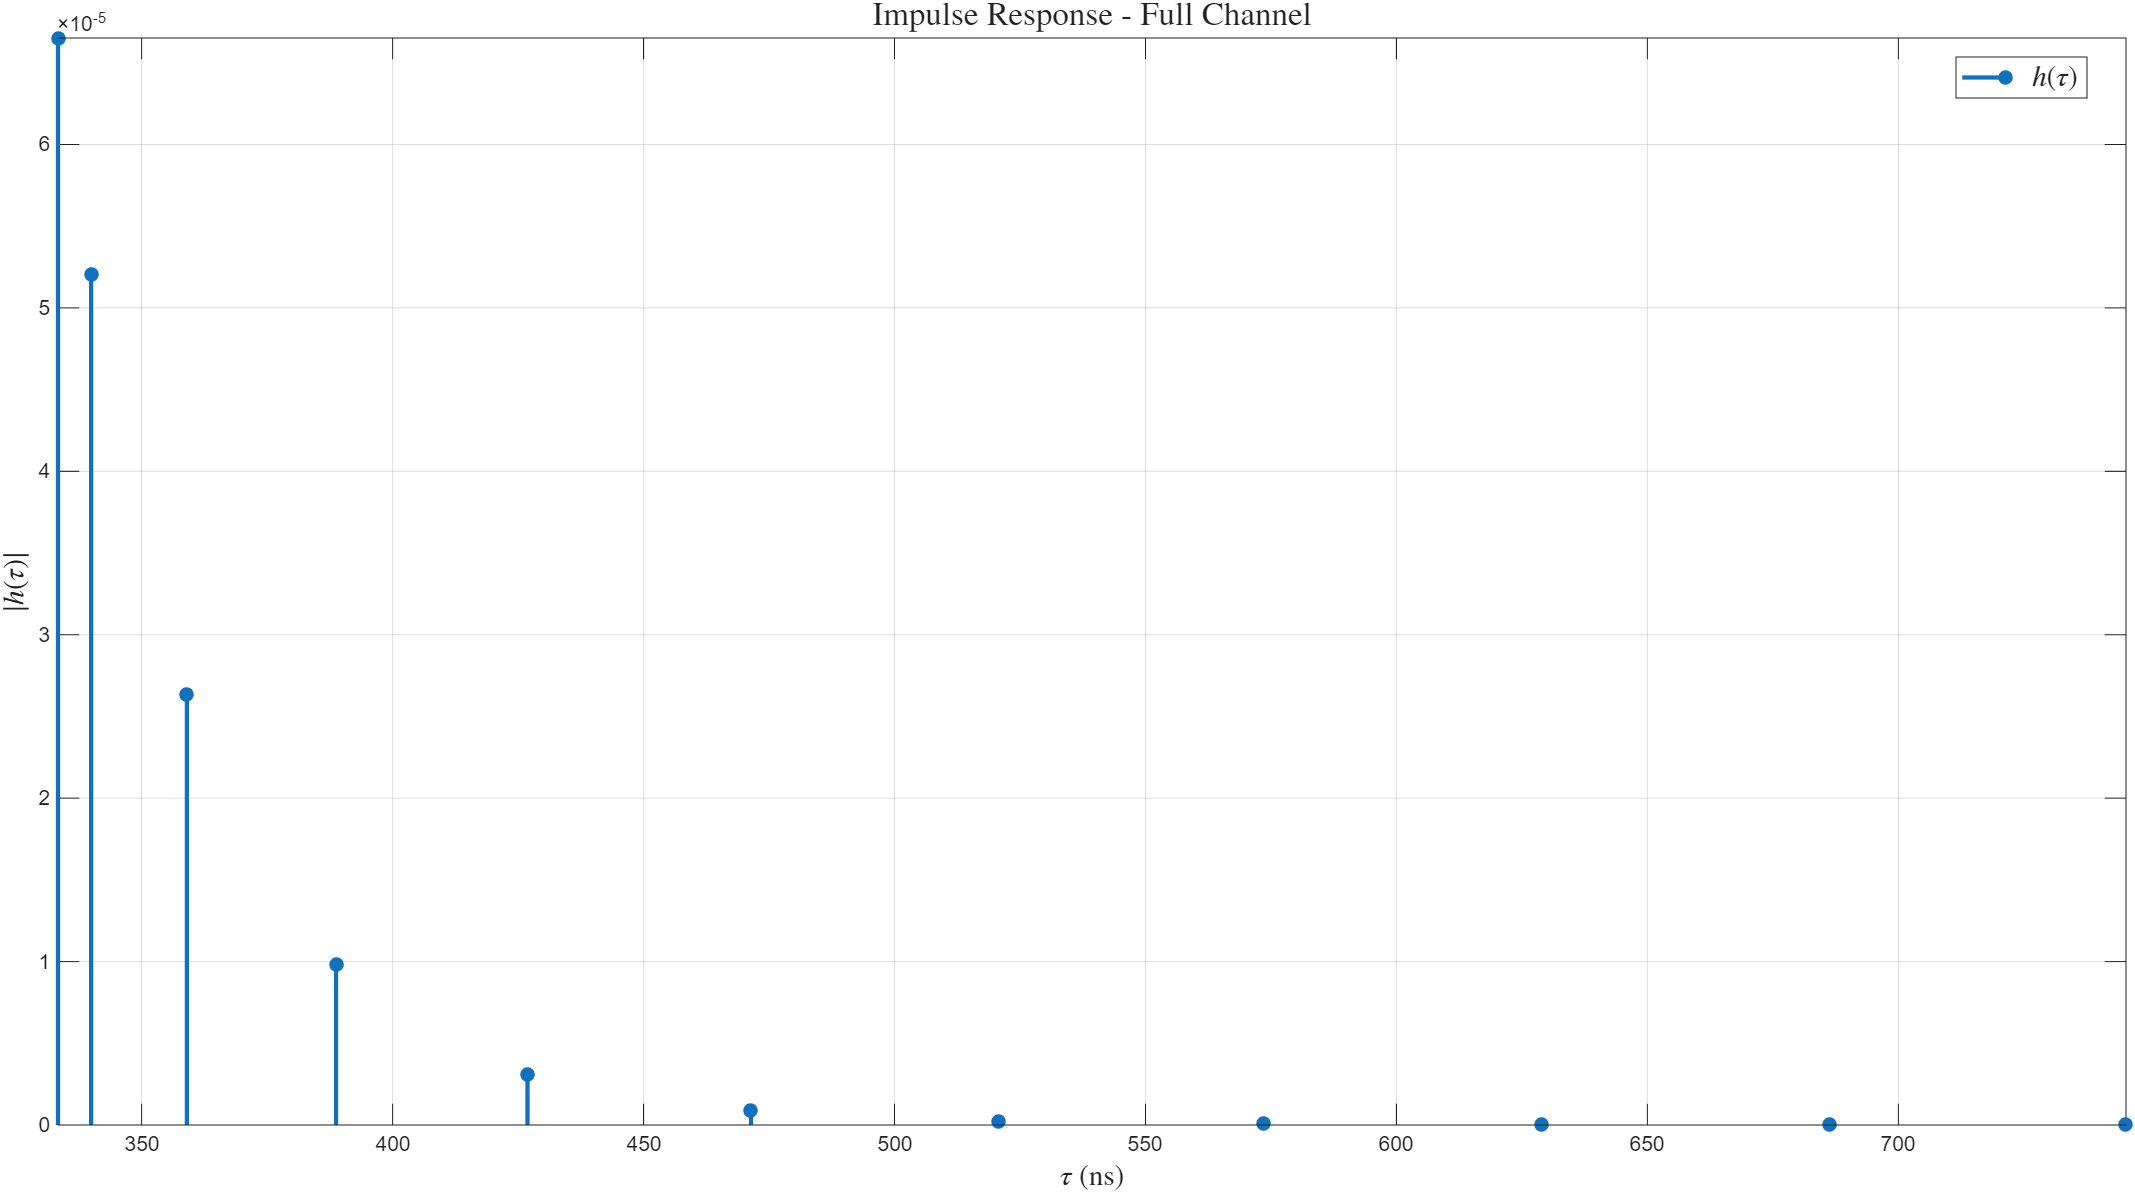
\includegraphics[width=\linewidth]{"content/4-images/h-tau - Full Channel.png"}
	\caption{Physical impulse response $|h(\tau)|$ for the full channel at $d=100$ m. The multiple impulses represent the various MPCs arriving at different delays, illustrating time dispersion.}
	\label{fig:h_tau_full}
\end{figure}

\section{Transfer Function $H(f)$}
The transfer function $H(f)$ is the Fourier transform of the physical impulse response $h(\tau)$:
\begin{align}
	H(f) &= \mathcal{FT}\left\{ \sum_{n=1}^{N} \alpha_n \delta(\tau - \tau_n) \right\} \\
	&= \sum_{n=1}^{N} \alpha_n \mathcal{FT}\left\{ \delta(\tau - \tau_n) \right\} \\
	&= \sum_{n=1}^{N} \alpha_n e^{-j2\pi f \tau_n}
	\label{eq:full_transfer_function_wide}
\end{align}
The transfer function is now a sum of complex phasors. As the frequency $f$ varies, the relative phases of these components change, leading to constructive and destructive interference. This causes the magnitude of the transfer function, $|H(f)|$, to vary significantly across the bandwidth, a phenomenon known as \textbf{frequency-selective fading}. As seen in Figure \ref{fig:Hf_full}, the channel exhibits deep nulls at frequencies where the MPCs combine destructively.

\begin{figure}[h!]
	\centering
	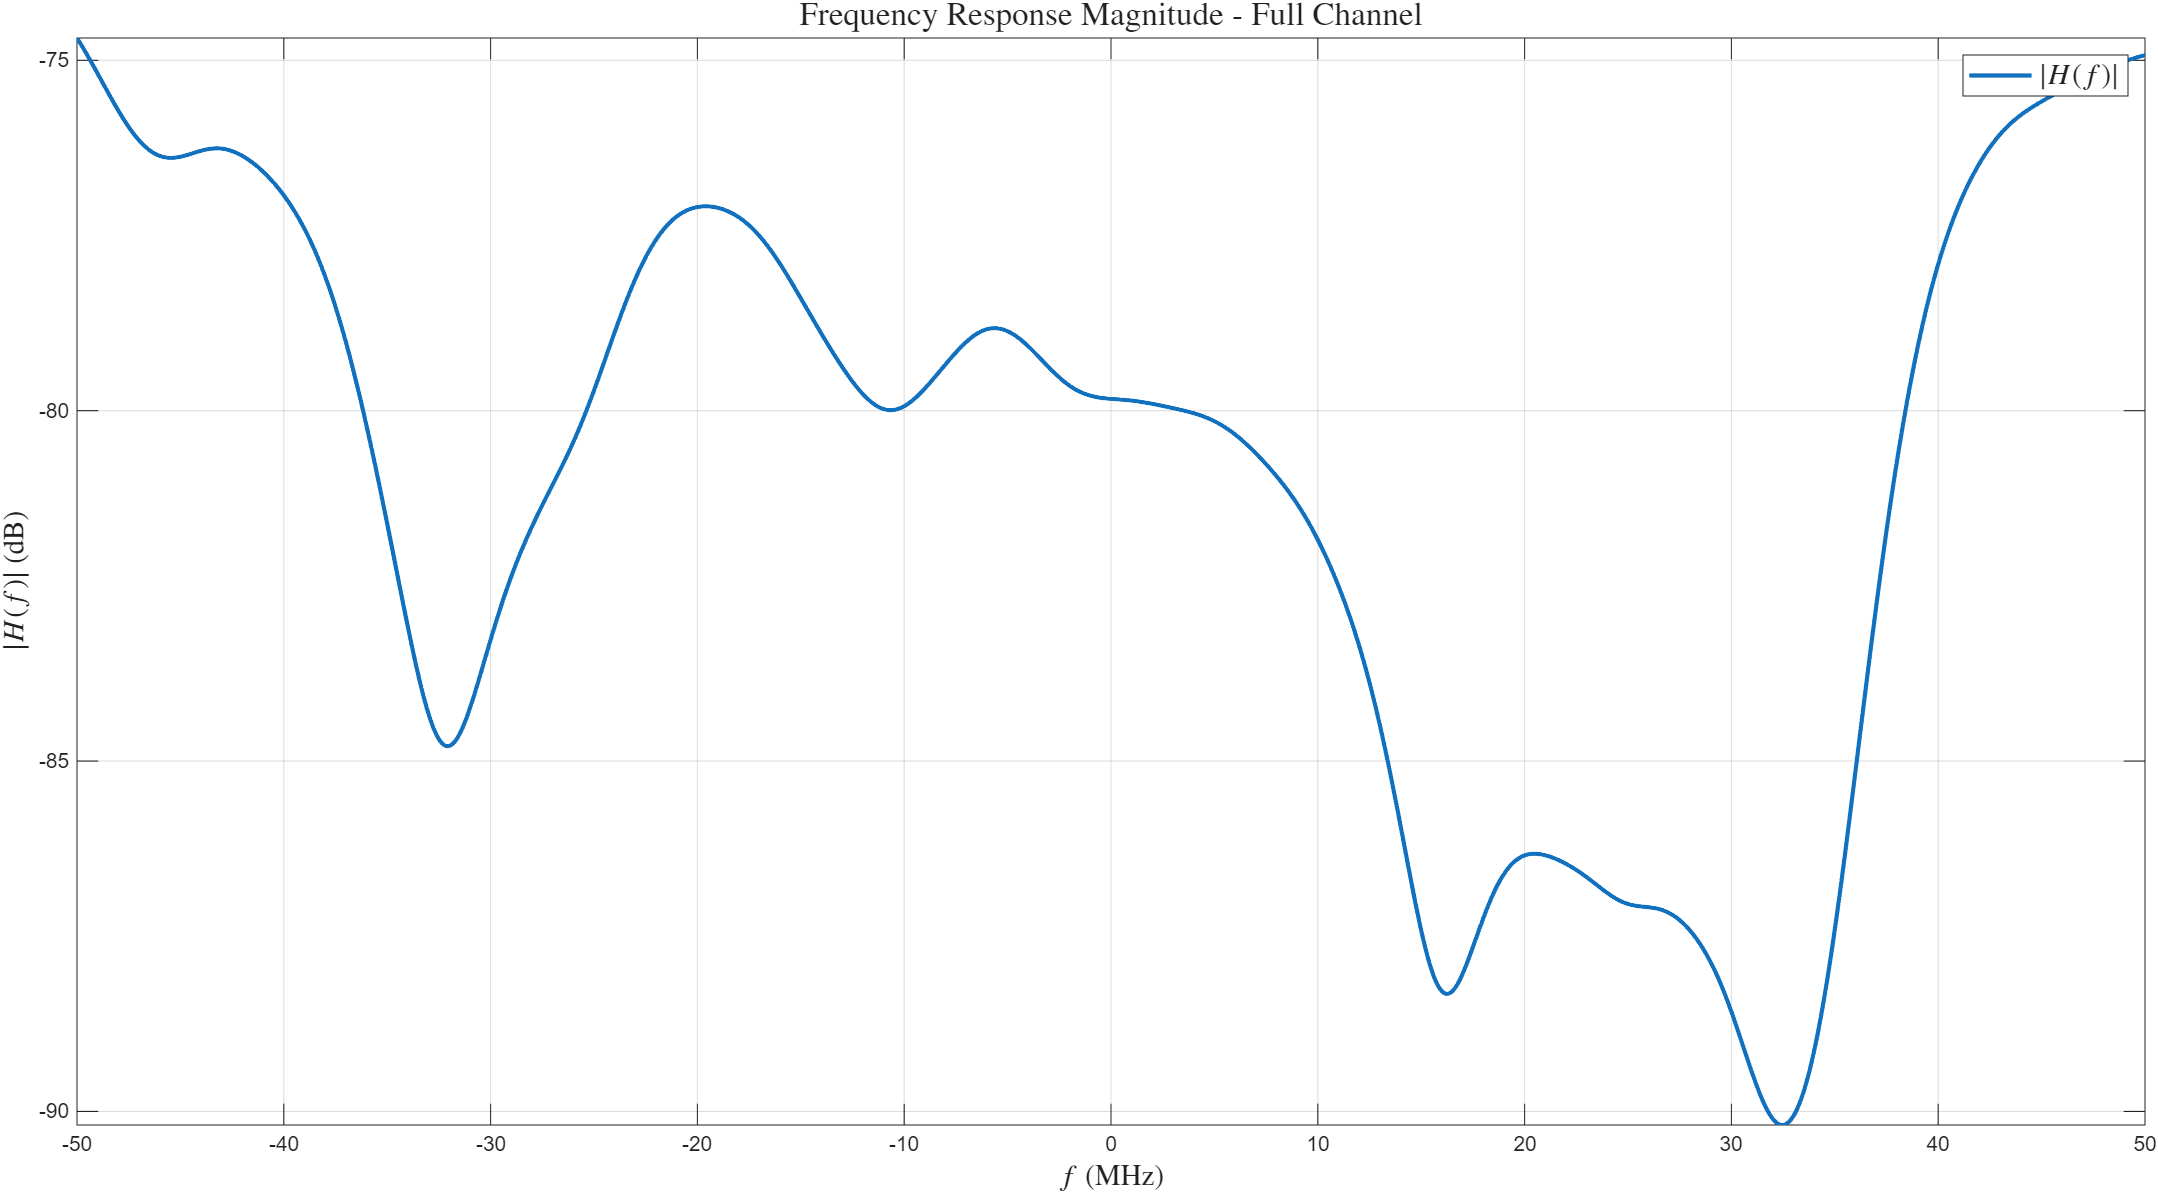
\includegraphics[width=\linewidth]{"content/4-images/Frequency Response H(f) - Full Channel.png"}
	\caption{Transfer function magnitude $|H(f)|$ for the full channel. The constructive and destructive interference of the MPCs creates deep nulls, illustrating frequency-selective fading.}
	\label{fig:Hf_full}
\end{figure}

\section{Tapped Delay Line Model $h_{TDL}(\tau)$}
As in the LOS case, the TDL model provides a practical, band-limited representation of the channel. The gain of the $l$-th tap, $h_l$, is found by integrating the full physical impulse response against the sinc function:
\begin{align}
	h_l &= \int_0^{\infty} h(\tau) \operatorname{sinc}(B(\tau-l \Delta \tau)) d \tau \\
	&= \int_0^{\infty} \left( \sum_{n=1}^{N} \alpha_n \delta(\tau - \tau_n) \right) \operatorname{sinc}(B(\tau-l \Delta \tau)) d \tau
\end{align}
Applying the sifting property of the delta function for each term in the sum yields:
\begin{equation}
	\boxed{h_l = \sum_{n=1}^{N} \alpha_n \operatorname{sinc}(B(\tau_n - l \Delta \tau))}
\end{equation}
Each tap gain $h_l$ is now a coherent sum of all physical MPCs, weighted by how close their delays $\tau_n$ are to the tap position $l\Delta\tau$. This model effectively groups the physical rays into discrete time bins, with the complex gain of each bin representing the vector sum of the rays falling within it. The resulting TDL impulse response, shown in Figure \ref{fig:h_tdl_full}, has significant energy spread across multiple taps, directly reflecting the time-dispersive nature of the physical channel.

\begin{figure}[h!]
	\centering
	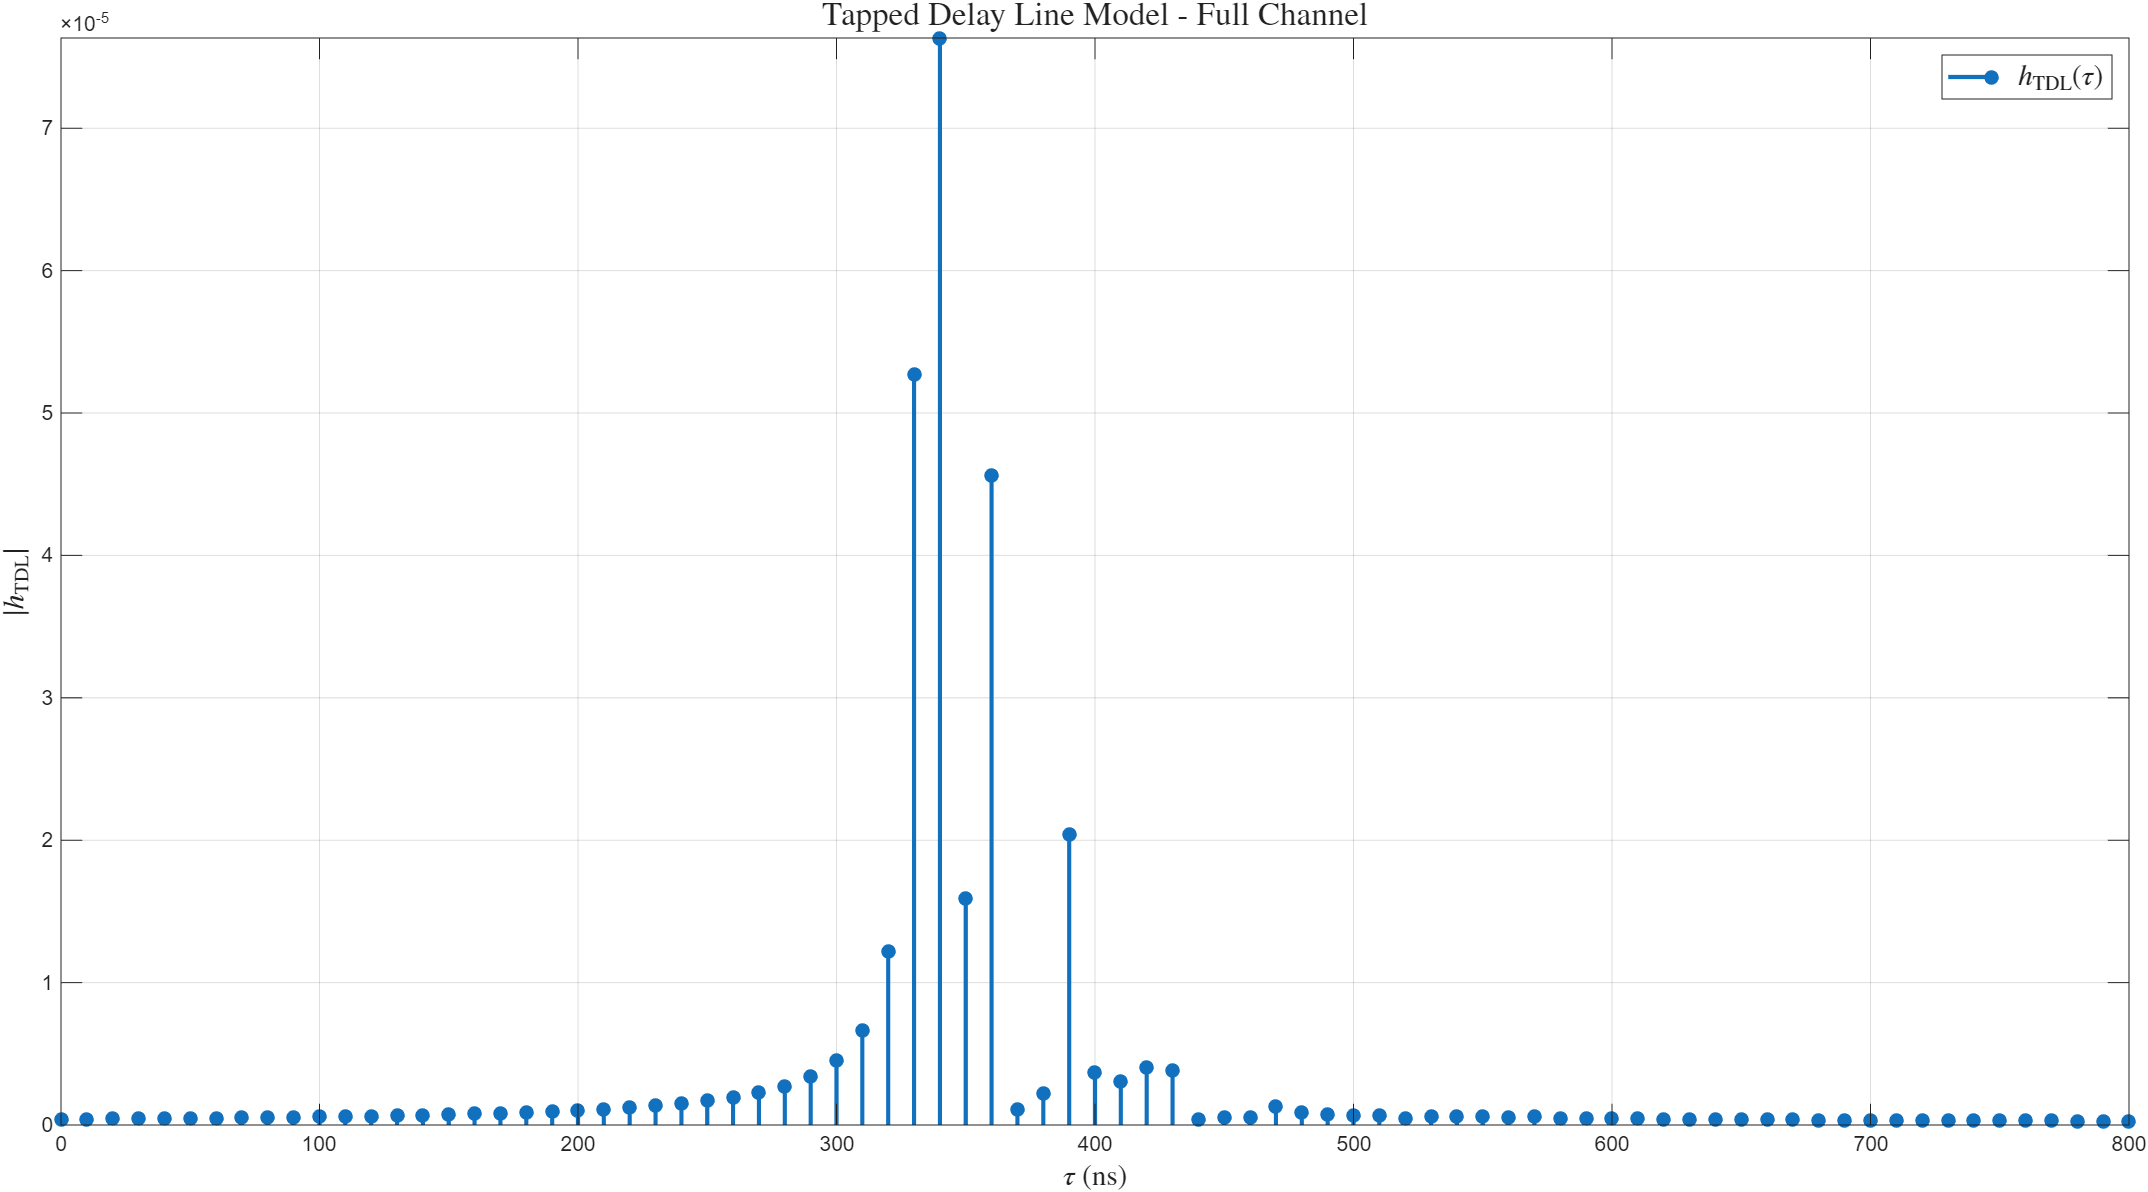
\includegraphics[width=\linewidth]{"content/4-images/Tapped Delay Line Model - Full Channel.png"}
	\caption{Tapped Delay Line model $|h_{TDL}(\tau)|$ for the full channel. The energy from the 21 MPCs is distributed across numerous taps, creating a discrete-time profile that mirrors the physical channel's delay spread.}
	\label{fig:h_tdl_full}
\end{figure}

\section{Interpretation of Results}
The wideband analysis of the full multiray channel reveals the fundamental challenges of wireless communication in such environments:
\begin{itemize}
	\item \textbf{Time Dispersion and Intersymbol Interference (ISI):} The physical impulse response in Figure \ref{fig:h_tau_full} shows that a transmitted impulse is received as a series of echoes spread out in time. This delay spread means that the energy from one transmitted symbol will spill over into the time slots of subsequent symbols, causing Intersymbol Interference (ISI). ISI is a major source of errors in digital communications and requires complex equalization techniques at the receiver to mitigate.
	\item \textbf{Frequency-Selective Fading:} The time dispersion is the direct cause of the frequency-selective fading observed in Figure \ref{fig:Hf_full}. The deep nulls in the channel's frequency response can completely wipe out parts of the signal's spectrum. If important information is located at these frequencies, it can be lost. This is why wideband systems often employ techniques like Orthogonal Frequency Division Multiplexing (OFDM), which divides the data into many narrow sub-carriers, making the system more robust to these selective fades.
	\item \textbf{TDL as a Practical Channel Model:} The TDL model (Figure \ref{fig:h_tdl_full}) is a powerful and practical tool. It captures the essential time-dispersive nature of the channel in a discrete format that is directly usable in system-level simulations and for designing digital equalizers. The number of significant taps in the TDL model is a direct measure of the severity of the channel's memory and the complexity required for the equalizer.
\end{itemize}
